\chapter{Desenvolvimento e Implementação}

Este capítulo apresenta a materialização do modelo proposto por meio de duas Provas de Conceito (PoC) complementares. A escolha por duas PoC responde a dois objetivos distintos e igualmente relevantes:

\begin{enumerate}
    \item \textbf{PoC AWS} (Seção~\ref{sec:poc-aws})~\citeonline{PocDevSecOpsAWS2026}: demonstra o modelo em um \textbf{ambiente corporativo real} de nuvem pública, com serviços gerenciados, federação de identidade, múltiplos ambientes e auditoria contínua. Ela representa o cenário para o qual o modelo foi originalmente concebido.
    \item \textbf{PoC de Contêineres} (Seção~\ref{sec:poc-containers})~\citeonline{PocDevSecOps2026}: espelha a mesma topologia lógica em ambiente \textbf{local, baseado em Docker}, com o objetivo de garantir \textbf{reprodutibilidade acadêmica} -- qualquer pessoa com Docker instalado consegue executar toda a esteira sem depender de conta em provedor de nuvem, sem incorrer em custos e sem exigir permissões elevadas em ambientes de terceiros.
\end{enumerate}

Ambas as PoC compartilham o mesmo modelo conceitual (Seção~\ref{sec:modelo}) e as mesmas ferramentas de análise, o que permite estabelecer uma correspondência direta entre ``o que a esteira faria em produção AWS'' e ``o que a esteira faz em uma máquina de estudante''. Todo o código-fonte discutido está publicamente disponível nos repositórios listados em~\citeonline{PocDevSecOps2026, PocDevSecOpsAWS2026}.

\section{Modelo Proposto}
\label{sec:modelo}

O modelo proposto se baseia na estratégia \textit{Shift-Left}~\citeonline{jimenez2019state}, deslocando os controles de segurança para as fases embrionárias do SDLC, garantindo que conformidade e resiliência sejam estabelecidas de forma nativa, mitigando riscos antes mesmo do provisionamento dos recursos em ambiente de nuvem. A esteira é organizada em cinco camadas hierárquicas de \textit{quality gates}~\citeonline{kim2021devops}:

\begin{enumerate}
    \item \textbf{Source (pré-commit e commit):} \textit{Pre-commit Hooks} locais executam \texttt{terraform fmt}, \textit{lint} de \textit{Dockerfiles}, formatação e detecção de segredos, impedindo que \textit{commits} defeituosos entrem no histórico do Git.
    \item \textbf{Build (CI - análise estática):} a pipeline valida o Terraform (\texttt{fmt}, \texttt{init}, \texttt{validate}, \textit{TFLint}), executa \textbf{Checkov} sobre HCL e \textit{Dockerfiles}, e faz uma segunda passagem de segredos (\textbf{Gitleaks} obrigatório, \textbf{ggshield} opcional se o segredo do GitGuardian estiver configurado).
    \item \textbf{Policy (Policy-as-Code):} o \texttt{terraform plan} é serializado em JSON e submetido ao \textbf{OPA/Conftest} contra políticas customizadas em \textit{Rego} (bloqueio de SSH público, IAM permissivo, IMDSv2, \textit{whitelist} de regiões, FinOps). Manifestos Kubernetes passam pelo mesmo motor.
    \item \textbf{Image hygiene:} \textbf{Hadolint} valida o \textit{Dockerfile} e \textbf{Trivy} escaneia o sistema de arquivos e as imagens em busca de CVEs e \textit{misconfigurations}.
    \item \textbf{Deploy e Operate:} apenas quando todos os \textit{gates} anteriores passam, o \texttt{terraform apply} (na PoC AWS, via \textit{role} assumida por OIDC) provisiona os recursos. Na PoC AWS, a auditoria contínua é apoiada por CloudTrail, AWS Config e Security Hub~\citeonline{AWS2026}.
\end{enumerate}

A Figura~\ref{fig:arquitetura-devsecops} sintetiza esse fluxo.

\begin{figure}[!ht]
    \caption{Arquitetura da esteira DevSecOps integrada, do código-fonte ao ambiente de nuvem, com portões de validação (SAST, SCA, Secrets, Policy-as-Code) atuando como barreiras de conformidade.}
    \label{fig:arquitetura-devsecops}
    \centering
    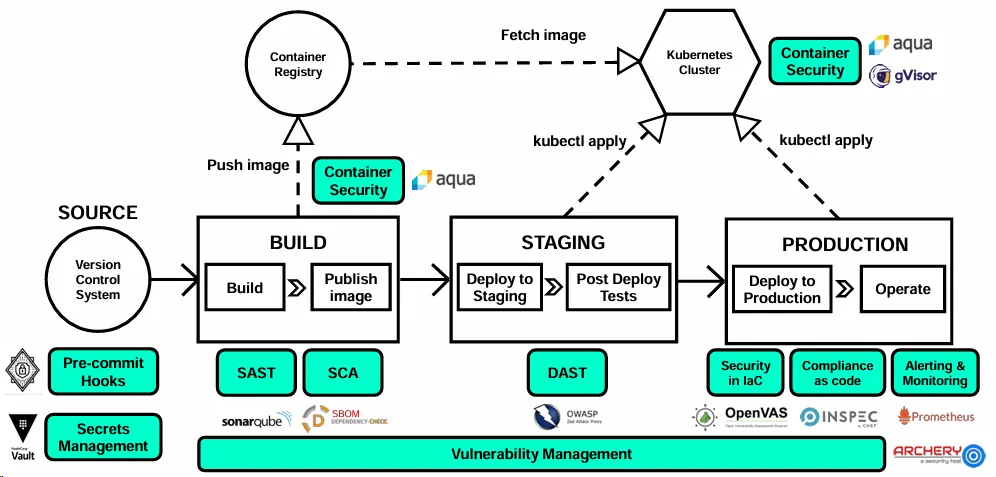
\includegraphics[width=0.85\textwidth]{Arquivos/figuras/Figura_Arquitetura_DevSecOps.png}
    \fonte{Elaborado pelo autor}
\end{figure}

Como observado no diagrama, a arquitetura foca na \textbf{visibilidade total} das falhas em cada camada. No início do fluxo (\textit{Source}), destacam-se os \textit{Pre-commit Hooks} e a gestão de segredos (\textit{Secrets Management}), que impedem a propagação de credenciais sensíveis. Durante o \textit{Build}, a análise estática (SAST) e a análise de composição de \textit{software} (SCA) garantem a integridade das bibliotecas e do código IaC, enquanto a segurança de contêineres e o monitoramento contínuo fecham o ciclo no ambiente de execução, produzindo uma infraestrutura resiliente e auditável.

\section{Cenário 1 -- PoC em Nuvem AWS}
\label{sec:poc-aws}

\subsection{Recursos AWS provisionados}

Para materializar o modelo em um cenário produtivo, a PoC AWS provisiona uma infraestrutura completa que reflete padrões corporativos, apoiada nos controles do CIS AWS Foundations~\citeonline{CIS2024AWS}:

\begin{itemize}
    \item \textbf{VPC dedicada} com CIDR parametrizável, sub-redes públicas (ALB), sub-redes privadas de aplicação (EKS) e sub-redes privadas de dados (RDS), distribuídas em múltiplas \textit{Availability Zones} (Seção~\ref{sec:fundamentos-rede});
    \item \textbf{VPC Flow Logs} em CloudWatch (CIS 3.9), \textbf{VPC Endpoints} para S3/KMS/Secrets Manager e restrição do \textit{default security group} e da \textit{default NACL} (CIS 5.3 e 5.4);
    \item \textbf{EKS} (\textit{Kubernetes} gerenciado) com \textit{node group} em sub-redes privadas, \textbf{IRSA} (\textit{IAM Roles for Service Accounts}) e criptografia via \textbf{KMS};
    \item \textbf{RDS PostgreSQL} multi-AZ em sub-redes privadas, com criptografia em repouso, \textit{backup} automatizado e credencial gerenciada via \textbf{Secrets Manager};
    \item \textbf{ECR} para imagens de contêiner, com \textit{scanning} habilitado;
    \item \textbf{S3} em três buckets (\texttt{artifacts}, \texttt{app-data}, \texttt{access-logs}), todos com SSE-KMS, \textit{public access block}, versionamento (quando aplicável) e negação de tráfego não criptografado;
    \item \textbf{Observabilidade e governança}: CloudTrail, AWS Config (com \textit{conformance pack} CIS), Security Hub com \textit{standards} CIS e AWS Foundational, opcionalmente SCPs de \textit{governance};
    \item \textbf{OIDC federado} para GitHub Actions, dispensando \texttt{AWS\_ACCESS\_KEY} de longa duração no repositório.
\end{itemize}

O trecho a seguir mostra a composição do ambiente \texttt{dev} da PoC AWS, no qual cada módulo é uma unidade coesa e isolada. Observa-se que a rede é a primeira dependência, seguida por segurança, IAM, dados e, por fim, computação (EKS).

\begin{lstlisting}[language=HCL,caption={Composição do ambiente \texttt{dev} na PoC AWS (\texttt{terraform/environments/dev/main.tf}). Ordem de resolução: KMS $\rightarrow$ Networking $\rightarrow$ IAM $\rightarrow$ Security $\rightarrow$ Storage $\rightarrow$ Secrets $\rightarrow$ Database $\rightarrow$ EKS.},label={lst:aws-envdev}]
module "kms" {
  source      = "../../modules/kms"
  name_prefix = local.name_prefix
  aws_region  = var.aws_region
  tags        = local.common_tags
}

module "networking" {
  source                   = "../../modules/networking"
  name_prefix              = local.name_prefix
  vpc_cidr                 = var.vpc_cidr
  availability_zones       = var.availability_zones
  az_count                 = length(var.availability_zones)
  enable_nat_gateway       = true
  enable_s3_endpoint       = true
  flow_logs_kms_key_arn    = module.kms.logs_key_arn
  flow_logs_retention_days = 30
  tags                     = local.common_tags
}

module "storage" {
  source           = "../../modules/storage"
  name_prefix      = local.name_prefix
  account_id       = local.account_id
  account_id_short = local.account_id_short
  kms_key_arn      = module.kms.s3_key_arn
  tags             = local.common_tags
}

module "eks" {
  source                    = "../../modules/eks"
  cluster_name              = local.cluster_name
  environment               = var.environment
  kubernetes_version        = var.kubernetes_version
  subnet_ids                = module.networking.app_subnet_ids
  cluster_role_arn          = module.iam.eks_cluster_role_arn
  cluster_security_group_id = module.security.eks_cluster_sg_id
  nodes_security_group_id   = module.security.eks_nodes_sg_id
  nodes_role_arn            = module.iam.eks_nodes_role_arn
  eks_kms_key_arn           = module.kms.eks_key_arn
  node_instance_types       = var.node_instance_types
  tags                      = local.common_tags
}
\end{lstlisting}

\subsection{Rede AWS: VPC modelada como código}

A modelagem da VPC é o alicerce da arquitetura, pois define o perímetro no qual todos os demais recursos existem. O módulo \texttt{networking} da PoC AWS provisiona uma VPC dedicada, distribuída em múltiplas AZ, com três camadas de sub-redes (pública, privada de aplicação e privada de dados). O Quadro~\ref{lst:aws-vpc} apresenta os principais elementos, com \textbf{VPC Flow Logs} (CIS AWS 3.9) e \textbf{IAM role} dedicado para o serviço \textit{vpc-flow-logs}.

\begin{lstlisting}[language=HCL,caption={Trecho do módulo \texttt{networking} da PoC AWS (\texttt{terraform/modules/networking/main.tf}): VPC com sub-redes por AZ, tabelas de rota separadas e VPC Flow Logs em CloudWatch.},label={lst:aws-vpc}]
resource "aws_vpc" "this" {
  cidr_block           = var.vpc_cidr
  enable_dns_support   = true
  enable_dns_hostnames = true

  tags = merge(var.tags, {
    Name      = "${var.name_prefix}-vpc"
    Simulates = "vpc-dockernetwork"
  })
}

resource "aws_subnet" "app" {
  count             = var.az_count
  vpc_id            = aws_vpc.this.id
  cidr_block        = local.app_subnets[count.index]
  availability_zone = local.azs[count.index]

  tags = merge(var.tags, {
    Name                              = "${var.name_prefix}-app-${local.azs[count.index]}"
    Tier                              = "private-app"
    "kubernetes.io/role/internal-elb" = "1"
  })
}

# --- VPC Flow Logs (CIS 3.9) ---
resource "aws_cloudwatch_log_group" "vpc_flow" {
  name              = "/aws/vpc/flow-logs/${var.name_prefix}"
  retention_in_days = var.flow_logs_retention_days
  kms_key_id        = var.flow_logs_kms_key_arn
  tags              = var.tags
}

resource "aws_flow_log" "this" {
  iam_role_arn         = aws_iam_role.vpc_flow.arn
  log_destination      = aws_cloudwatch_log_group.vpc_flow.arn
  log_destination_type = "cloud-watch-logs"
  traffic_type         = "ALL"
  vpc_id               = aws_vpc.this.id
}
\end{lstlisting}

A Figura~\ref{fig:vpc-console} apresenta a visualização, no console AWS, da VPC efetivamente provisionada por essa configuração, servindo como evidência empírica de que o \textit{plan} foi aplicado com sucesso.

\begin{figure}[!ht]
    \caption{VPC provisionada via IaC no console AWS. O bloco CIDR observado no console corresponde àquele declarado no código Terraform, evidenciando a integridade do processo automatizado.}
    \label{fig:vpc-console}
    \centering
    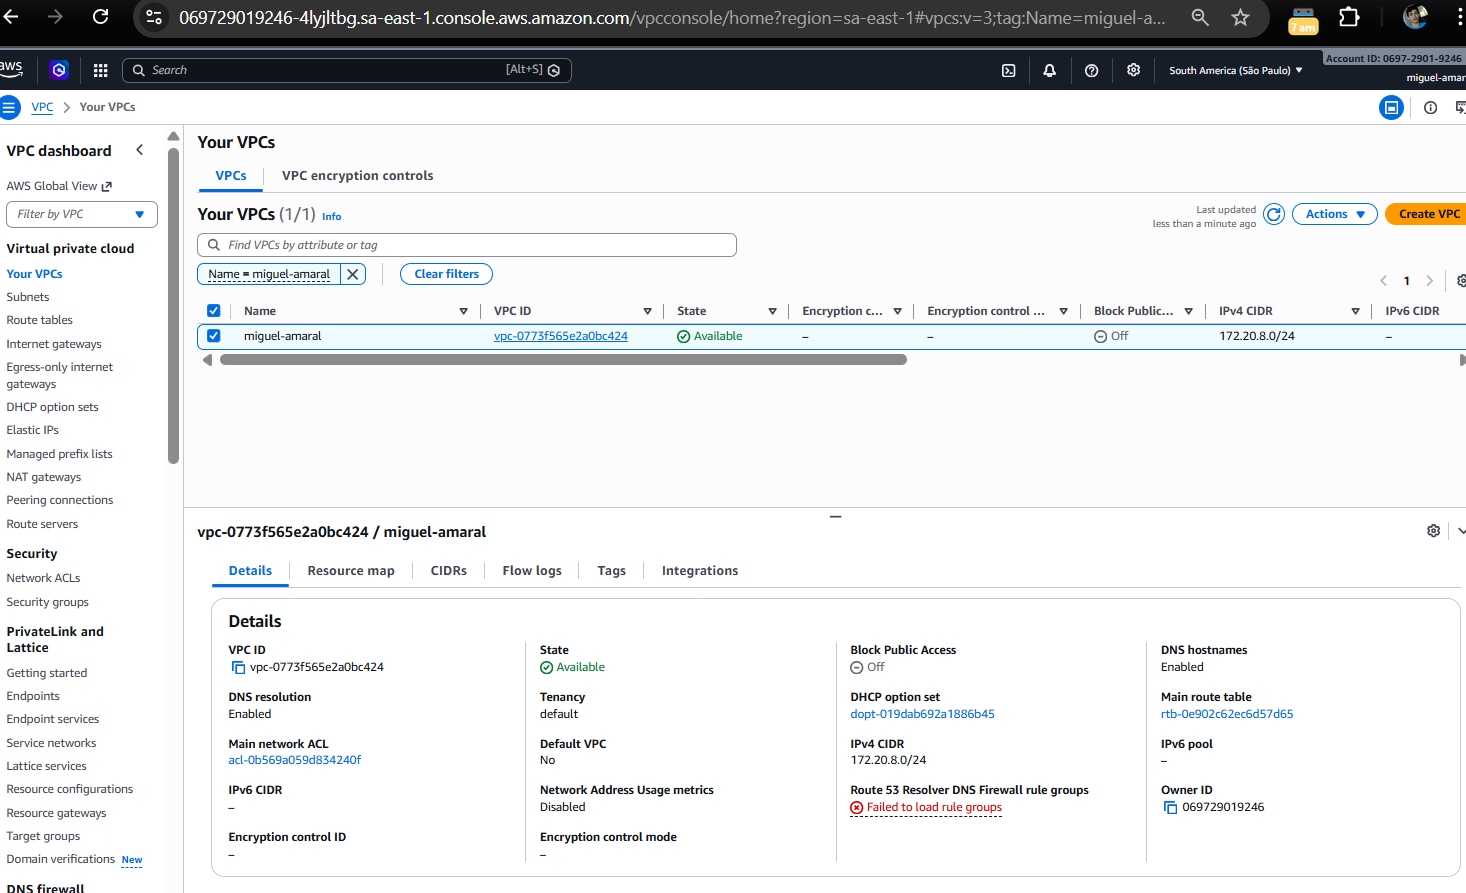
\includegraphics[width=0.8\textwidth]{Arquivos/figuras/Figura_VPC_Dashboard_AWS.png}
    \fonte{Elaborado pelo autor}
\end{figure}

\subsection{Armazenamento seguro: buckets S3 com controles nativos}

O módulo \texttt{storage} materializa quatro controles do CIS AWS Foundations em uma única definição declarativa: (i) \texttt{aws\_s3\_bucket\_public\_access\_block} bloqueando qualquer forma de acesso público (CIS 2.1.5); (ii) \texttt{aws\_s3\_bucket\_server\_side\_encryption\_configuration} com SSE-KMS obrigatório (CIS 2.1.1); (iii) \texttt{aws\_s3\_bucket\_versioning} para objetos sensíveis; e (iv) políticas de bucket que negam tráfego não criptografado (\texttt{aws:SecureTransport = false}).

\begin{lstlisting}[language=HCL,caption={Configuração declarativa de segurança para buckets S3 (\texttt{terraform/modules/storage/main.tf}).},label={lst:aws-s3}]
resource "aws_s3_bucket_public_access_block" "this" {
  for_each = local.buckets

  bucket                  = aws_s3_bucket.this[each.key].id
  block_public_acls       = true
  block_public_policy     = true
  ignore_public_acls      = true
  restrict_public_buckets = true
}

resource "aws_s3_bucket_server_side_encryption_configuration" "this" {
  for_each = local.buckets

  bucket = aws_s3_bucket.this[each.key].id

  rule {
    apply_server_side_encryption_by_default {
      sse_algorithm     = "aws:kms"
      kms_master_key_id = var.kms_key_arn
    }
    bucket_key_enabled = true
  }
}
\end{lstlisting}

\subsection{Esteira DevSecOps em GitHub Actions}
\label{sec:pipeline-aws}

A pipeline da PoC AWS (arquivo \texttt{.github/workflows/security-scan.yml}) implementa os cinco \textit{quality gates} descritos na Seção~\ref{sec:modelo}. Cada \textit{job} depende do anterior (\texttt{needs:}), o que garante o comportamento \textit{Fail-Fast}: se \textbf{secrets} falhar, os demais nem chegam a executar. O Quadro~\ref{lst:aws-pipeline} apresenta os \textit{jobs} de detecção de segredos e de análise estática de Terraform.

\begin{lstlisting}[language=yaml,caption={Trecho da pipeline \texttt{security-scan.yml} (PoC AWS): detecção de segredos com Gitleaks (obrigatório) e ggshield (opcional), seguida de \texttt{fmt}, \texttt{validate}, \texttt{tflint} e \texttt{Checkov} em matriz de ambientes.},label={lst:aws-pipeline}]
jobs:
  secrets:
    name: 1. Secrets (gitleaks + ggshield)
    runs-on: ubuntu-latest
    env:
      GG_KEY_SET: ${{ secrets.GITGUARDIAN_API_KEY != '' }}
    steps:
      - uses: actions/checkout@v4
        with: { fetch-depth: 0 }
      - name: Run gitleaks
        uses: gitleaks/gitleaks-action@v2
        env:
          GITLEAKS_CONFIG: ${{ github.workspace }}/.gitleaks.toml
      - name: Run ggshield (GitGuardian)
        if: env.GG_KEY_SET == 'true'
        uses: GitGuardian/ggshield-action@v1
        env:
          GITGUARDIAN_API_KEY: ${{ secrets.GITGUARDIAN_API_KEY }}

  terraform-static:
    name: 2. Terraform static checks (fmt, validate, tflint, checkov)
    runs-on: ubuntu-latest
    needs: secrets
    strategy:
      fail-fast: false
      matrix:
        env: [dev, prod]
    steps:
      - uses: actions/checkout@v4
      - uses: hashicorp/setup-terraform@v3
        with: { terraform_version: 1.9.0, terraform_wrapper: false }
      - run: terraform -chdir=terraform fmt -check -recursive
      - name: terraform init (no backend)
        working-directory: terraform/environments/${{ matrix.env }}
        run: terraform init -backend=false
      - name: terraform validate
        working-directory: terraform/environments/${{ matrix.env }}
        run: terraform validate
      - name: Checkov scan
        run: |
          checkov --config-file policies/checkov/.checkov.yaml \
                  --output cli --output sarif --output-file-path .
      - name: Upload SARIF
        if: always()
        uses: github/codeql-action/upload-sarif@v3
        with: { sarif_file: results_sarif.sarif }
\end{lstlisting}

Duas decisões merecem destaque:

\begin{itemize}
    \item \textbf{Camadas OSS + SaaS para segredos:} Gitleaks (código aberto) é obrigatório em todas as execuções; ggshield (GitGuardian) roda apenas quando o segredo \texttt{GITGUARDIAN\_API\_KEY} está configurado, o que permite executar a pipeline em \textit{forks} públicos sem interrupções.
    \item \textbf{Matriz por ambiente:} os \textit{jobs} de Terraform e OPA rodam em paralelo para \texttt{dev} e \texttt{prod}, aumentando a cobertura sem duplicação de código.
\end{itemize}

\subsection{Policy-as-Code: OPA/Rego contra o \texttt{terraform plan}}

Diferentemente do Checkov -- que aplica regras genéricas ao HCL --, o OPA analisa o \textbf{plano de execução} do Terraform já resolvido (o JSON de \texttt{terraform show}). Isso torna as políticas capazes de raciocinar sobre valores computados, dependências e o resultado final da alteração. A política a seguir bloqueia qualquer \textit{Security Group} que exponha SSH (porta 22) ou RDP (porta 3389) para \texttt{0.0.0.0/0}, cobrindo os formatos \texttt{aws\_vpc\_security\_group\_ingress\_rule} e \texttt{aws\_security\_group} (com \textit{ingress inline}).

\begin{lstlisting}[language=Rego,caption={Política OPA/Rego \texttt{deny\_public\_ssh.rego} (PoC AWS): bloqueio de SSH e RDP expostos à Internet, atendendo ao CIS AWS 5.2.},label={lst:opa-ssh}]
package terraform.security

import rego.v1

sg_rules contains rule if {
    some rc in input.resource_changes
    rc.type in {"aws_security_group", "aws_vpc_security_group_ingress_rule"}
    rc.change.actions[_] in {"create", "update"}
    rule := rc.change.after
}

deny contains msg if {
    some r in sg_rules
    r.cidr_ipv4 == "0.0.0.0/0"
    port_in_range(r.from_port, r.to_port, 22)
    msg := sprintf("CIS 5.2: SSH (22) exposto a 0.0.0.0/0 em SG rule: %v", [r])
}

deny contains msg if {
    some rc in input.resource_changes
    rc.type == "aws_security_group"
    rc.change.actions[_] in {"create", "update"}
    some ing in rc.change.after.ingress
    "0.0.0.0/0" in ing.cidr_blocks
    port_in_range(ing.from_port, ing.to_port, 22)
    msg := sprintf("CIS 5.2: SSH (22) exposto a 0.0.0.0/0 em SG %q (inline)", [rc.address])
}

port_in_range(from, to, port) if {
    is_number(from); is_number(to)
    port >= from; port <= to
}
\end{lstlisting}

Outra política, dedicada à governança financeira (\textit{FinOps}), bloqueia famílias de instância caras em ambientes não-produtivos, aplicando o conceito de governança como código~\citeonline{OPA2024}:

\begin{lstlisting}[language=Rego,caption={Política OPA/Rego \texttt{finops\_instance\_types.rego}: bloqueia \textit{instance types} caros em ambientes não-produtivos.},label={lst:opa-finops}]
package terraform.finops

import rego.v1

forbidden_instance_patterns := [
    "^p[2-5]\\.",      # aceleradas por GPU
    "^x[12].*\\.",     # memoria extra-alta
    "^u-.*",           # dedicated hosts (u-24tb1 etc.)
    "\\.24xlarge$", "\\.32xlarge$", "\\.48xlarge$", "\\.metal$",
]

deny contains msg if {
    some rc in input.resource_changes
    rc.type == "aws_instance"
    rc.change.actions[_] in {"create", "update"}
    instance_type := rc.change.after.instance_type
    some pattern in forbidden_instance_patterns
    regex.match(pattern, instance_type)
    is_non_prod(rc)
    msg := sprintf("FinOps: instance_type %q proibido em ambiente nao-producao (%q)",
                   [instance_type, rc.address])
}

is_non_prod(rc) if {
    tags := object.get(rc.change.after, "tags", {})
    env := lower(object.get(tags, "Environment", "dev"))
    env != "prod"; env != "production"
}
\end{lstlisting}

Políticas análogas foram implementadas para: negação de IAM \textit{admin-total} (\texttt{Action="*"} + \texttt{Resource="*"}), imposição de IMDSv2 em EC2/Launch Templates, negação de RDS/EBS sem criptografia, \textit{whitelist} de regiões (LGPD) e \textit{enforcement} de \textit{tags}~\citeonline{PocDevSecOpsAWS2026}.

\subsection{Verificações Checkov selecionadas}

A matriz de políticas Checkov utilizada é sintetizada na Tabela~\ref{tab:checkov} (originalmente registrada por meio de imagem, mantida por conveniência). A escolha das regras seguiu dois critérios: (i) severidade \textit{Critical}/\textit{High} nos \textit{benchmarks}; e (ii) recorrência do problema em relatórios de mercado como o~\citeonline{ibmDataBreachCost}.

\begin{table}[!ht]
    \caption{Matriz de políticas de segurança e conformidade configuradas no Checkov, correlacionando recursos AWS aos identificadores de regras (CIS Benchmarks) e à severidade adotada.}
    \label{tab:checkov}
    \centering
    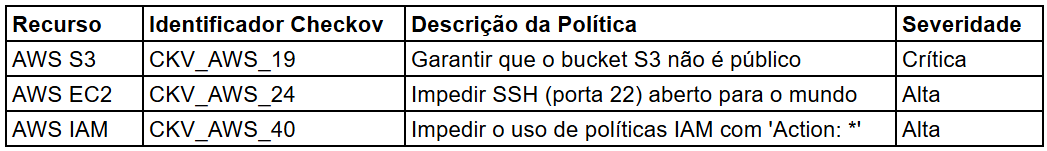
\includegraphics[width=0.8\textwidth]{Arquivos/figuras/Tabela_Verificacoes_Seguranca_Checkov.png}
    \fonte{Elaborado pelo autor}
\end{table}

\subsection{Detecção de segredos em duas camadas}

A gestão de segredos é implementada em três pontos, refletindo a \textit{defense-in-depth}~\citeonline{OWASPCheatSheet}:

\begin{itemize}
    \item \textbf{Pre-commit local:} \texttt{gitleaks protect} bloqueia o \textit{commit} antes de entrar no histórico;
    \item \textbf{CI OSS:} Gitleaks executa no \textit{job} \texttt{secrets} da pipeline com um \texttt{.gitleaks.toml} customizado que reduz falsos positivos (por exemplo, \texttt{account\_id} em código de exemplo);
    \item \textbf{CI SaaS:} ggshield (GitGuardian) roda em paralelo quando a credencial está disponível, agregando análise contextual e o histórico do repositório.
\end{itemize}

Diferentemente das ferramentas de análise de configuração, o GitGuardian especializa-se na identificação proativa de informações sensíveis expostas -- como chaves de API da AWS, certificados digitais e credenciais de bancos de dados -- que poderiam ser inadvertidamente incluídas no histórico do repositório. A detecção precoce desses ativos é fundamental, pois, uma vez que um segredo é enviado ao repositório, sua invalidação e a limpeza do histórico do Git tornam-se processos complexos e onerosos~\citeonline{OWASPCheatSheet}. Mesmo que o código seja removido em um \textit{commit} posterior, o segredo permanece acessível no histórico de revisões, exigindo a revogação imediata da credencial para mitigar riscos de exploração.

\subsection{Kubernetes: NetworkPolicies e políticas em Rego}

Como o EKS (Kubernetes) é o \textit{workload}, aplicaram-se controles adicionais no plano do \textit{cluster}: \textit{NetworkPolicies} \textit{default-deny} com permissões explícitas para o tráfego desejado (CIS K8s 5.3) e políticas OPA que bloqueiam \textit{privileged containers} e \textit{privilege escalation} (CIS K8s 5.2.1/5.2.5).

\begin{lstlisting}[language=yaml,caption={\textit{NetworkPolicy} \textit{default-deny-all} no \textit{namespace} da aplicação (\texttt{k8s/manifests/50-network-policies.yaml}).},label={lst:k8s-netpol}]
apiVersion: networking.k8s.io/v1
kind: NetworkPolicy
metadata:
  name: default-deny-all
  namespace: app
spec:
  podSelector: {}
  policyTypes: [Ingress, Egress]
---
apiVersion: networking.k8s.io/v1
kind: NetworkPolicy
metadata:
  name: allow-backend-egress
  namespace: app
spec:
  podSelector:
    matchLabels: { app: backend-api }
  policyTypes: [Ingress, Egress]
  ingress:
    - from:
        - podSelector: { matchLabels: { app: frontend-nginx } }
      ports: [{ protocol: TCP, port: 8000 }]
  egress:
    # PostgreSQL no RDS (restringido pelo SG na rede)
    - to: [{ ipBlock: { cidr: 10.20.0.0/16 } }]
      ports: [{ protocol: TCP, port: 5432 }]
\end{lstlisting}

\begin{lstlisting}[language=Rego,caption={Política OPA \texttt{no\_privileged\_containers.rego}: bloqueia \textit{privileged}, \textit{hostNetwork}, \textit{hostPID}, \textit{hostIPC} e \textit{allowPrivilegeEscalation}.},label={lst:k8s-priv}]
package kubernetes.privileged

import rego.v1

containers contains c if {
    input.kind in {"Pod", "Deployment", "StatefulSet", "DaemonSet"}
    c := pod_spec(input).containers[_]
}

deny contains msg if {
    some c in containers
    c.securityContext.privileged == true
    msg := sprintf("CIS K8s 5.2.1: container %q em %q privileged=true",
                   [c.name, input.metadata.name])
}

deny contains msg if {
    some c in containers
    c.securityContext.allowPrivilegeEscalation == true
    msg := sprintf("CIS K8s 5.2.5: container %q permite privilege escalation", [c.name])
}

pod_spec(obj) := obj.spec if obj.kind == "Pod"
pod_spec(obj) := obj.spec.template.spec if obj.kind in {"Deployment", "StatefulSet", "DaemonSet"}
\end{lstlisting}

\section{Cenário 2 -- PoC Local com Contêineres (Reprodutibilidade)}
\label{sec:poc-containers}

A PoC de contêineres foi concebida como uma \textbf{tradução fiel} da arquitetura AWS para um ambiente local baseado em Docker. Ela cumpre três funções neste trabalho:

\begin{enumerate}
    \item \textbf{Reprodutibilidade acadêmica:} qualquer avaliador ou estudante pode executar toda a pipeline em uma máquina pessoal com Docker, sem necessidade de conta AWS, sem custos e sem exposição a riscos operacionais~\citeonline{PocDevSecOps2026};
    \item \textbf{Ensino:} facilita a compreensão dos conceitos de DevSecOps + IaC ao remover a camada de abstração da nuvem, permitindo inspecionar processos, redes e \textit{logs} localmente;
    \item \textbf{Base para migração:} ao manter os mesmos módulos Terraform (com \textit{provider} \texttt{docker} no lugar do \texttt{aws}), demonstra que o modelo é \textbf{provider-agnostic} em seu núcleo lógico, mesmo que os controles concretos difiram.
\end{enumerate}

\subsection{Mapeamento AWS $\rightarrow$ Docker}

A Tabela~\ref{tab:map-aws-docker} apresenta a correspondência conceitual entre os serviços da AWS e seus equivalentes em Docker adotados na PoC de contêineres.

\begin{table}[!ht]
\centering
\caption{Mapeamento entre serviços AWS e equivalentes em Docker adotados na PoC local}
\label{tab:map-aws-docker}
\renewcommand{\arraystretch}{1.3}
\begin{tabular}{|p{4.0cm}|p{4.5cm}|p{5.5cm}|}
\hline
\textbf{Conceito} & \textbf{AWS real (PoC AWS)} & \textbf{PoC de contêineres} \\
\hline
Isolamento de rede & VPC + sub-redes + tabelas de rota & \texttt{docker\_network} (\texttt{bridge}) com IPAM /16 dedicado \\
\hline
Camada de dados & Amazon RDS (PostgreSQL) multi-AZ & Contêiner \texttt{postgres:16-alpine} + volume nomeado \\
\hline
Camada de aplicação & EKS (\textit{node group}) + IRSA & N réplicas de \texttt{docker\_container} (FastAPI), com \texttt{count} \\
\hline
\textit{Load balancer} & Application Load Balancer + WAF & Contêiner \texttt{nginx-unprivileged} (proxy reverso e balanceador) \\
\hline
Gestão de segredos & Secrets Manager + IRSA & Variáveis \texttt{.env} + \texttt{TF\_VAR\_*} (nunca versionadas) \\
\hline
Observabilidade & CloudTrail / Config / Security Hub & \texttt{docker logs} + \textit{outputs} do Terraform \\
\hline
\end{tabular}
\fonte{Elaborado pelo autor}
\end{table}

A Figura~\ref{fig:arquitetura-containers} ilustra a topologia local, na qual todos os contêineres estão conectados a uma única \texttt{docker\_network}, simulando uma VPC única.

\begin{figure}[!ht]
    \caption{Arquitetura da PoC baseada em contêineres, com Nginx como \textit{load balancer} (\textit{ELB-NGINX}), múltiplas réplicas FastAPI (\textit{EKS-FASTAPI-XX}) e PostgreSQL (\textit{RDS-POSTGRES}), todos conectados à \texttt{VPC-DOCKERNETWORK}.}
    \label{fig:arquitetura-containers}
    \centering
    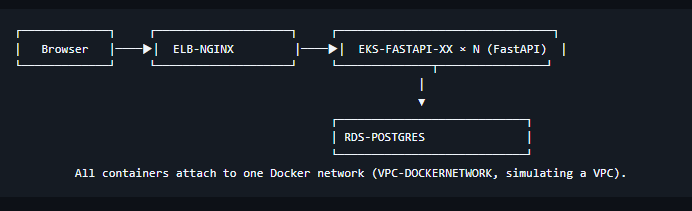
\includegraphics[width=0.75\textwidth]{Arquivos/figuras/Figura_Arquitetura_PoC_Containers.png}
    \fonte{Elaborado pelo autor}
\end{figure}

A convenção de nomes (\texttt{VPC-DOCKERNETWORK}, \texttt{RDS-POSTGRES}, \texttt{EKS-FASTAPI-01}, \texttt{ELB-NGINX}) foi deliberadamente escolhida para reforçar visualmente a analogia com AWS quando o leitor inspeciona a saída de \texttt{docker ps}.

\subsection{Módulos Terraform equivalentes}

O código HCL da PoC local mantém a mesma organização modular (\texttt{network}, \texttt{database}, \texttt{backend}, \texttt{frontend}), agora com o \textit{provider} \texttt{kreuzwerker/docker}. O Quadro~\ref{lst:docker-network} apresenta o módulo de rede: uma \texttt{docker\_network} com \textit{driver bridge}, IPAM em \texttt{172.28.0.0/16} e \textit{labels} que explicitam a simulação da VPC.

\begin{lstlisting}[language=HCL,caption={Módulo \texttt{network} da PoC de contêineres (\texttt{terraform/modules/network/main.tf}).},label={lst:docker-network}]
resource "docker_network" "this" {
  name   = "VPC-DOCKERNETWORK"
  driver = "bridge"

  ipam_config { subnet = "172.28.0.0/16" }

  labels {
    label = "environment"
    value = "local-poc"
  }
  labels {
    label = "simulates"
    value = "aws-vpc"
  }
}
\end{lstlisting}

O módulo \texttt{backend} (Quadro~\ref{lst:docker-backend}) provisiona múltiplas réplicas da API FastAPI (equivalentes lógicos dos \textit{pods} em EKS), com \texttt{privileged = false}, \textit{HEALTHCHECK} obrigatório e \textit{labels} que refletem a intenção original (\textit{role=backend}, \textit{replica=N}).

\begin{lstlisting}[language=HCL,caption={Módulo \texttt{backend} da PoC de contêineres: N réplicas FastAPI com \textit{HEALTHCHECK}, sem privilégios elevados e integradas à \texttt{docker\_network} única.},label={lst:docker-backend}]
resource "docker_container" "api" {
  count = var.replica_count

  name  = "EKS-FASTAPI-${format("%02d", count.index + 1)}"
  image = docker_image.backend.image_id

  restart    = "unless-stopped"
  privileged = false   # baseline de seguranca

  env = [
    "PGHOST=${var.db_host}",
    "PGPORT=${tostring(var.db_port)}",
    "PGUSER=${var.postgres_user}",
    "PGPASSWORD=${var.postgres_password}",
    "PGDATABASE=${var.postgres_db}",
  ]

  networks_advanced { name = var.network_id }

  healthcheck {
    test     = ["CMD-SHELL", "curl -fsS http://127.0.0.1:8000/health || exit 1"]
    interval = "15s"
    timeout  = "5s"
    retries  = 5
  }

  labels { label = "role"    value = "backend" }
  labels { label = "replica" value = tostring(count.index) }
}
\end{lstlisting}

O \textit{Dockerfile} do \textit{backend} incorpora as correções de segurança discutidas na Seção~\ref{sec:pipeline-containers}: usuário não-\textit{root}, \textit{HEALTHCHECK} e limpeza do cache do gerenciador de pacotes.

\begin{lstlisting}[language=dockerfile,caption={\textit{Dockerfile} do serviço FastAPI (\texttt{app/backend/Dockerfile}) da PoC de contêineres.},label={lst:dockerfile-backend}]
FROM python:3.12-slim-bookworm
WORKDIR /app

RUN apt-get update && apt-get install -y --no-install-recommends curl ca-certificates \
    && rm -rf /var/lib/apt/lists/* \
    && update-ca-certificates

COPY requirements.txt .
RUN pip install --no-cache-dir -r requirements.txt

COPY main.py .

RUN useradd --create-home --uid 1000 appuser \
    && chown -R appuser:appuser /app
USER appuser

ENV PYTHONUNBUFFERED=1
EXPOSE 8000
HEALTHCHECK --interval=15s --timeout=5s --retries=5 \
    CMD curl -fsS http://127.0.0.1:8000/health || exit 1

CMD ["uvicorn", "main:app", "--host", "0.0.0.0", "--port", "8000"]
\end{lstlisting}

\subsection{Esteira DevSecOps na PoC de contêineres}
\label{sec:pipeline-containers}

A pipeline da PoC de contêineres (\texttt{.github/workflows/pipeline.yml}) reproduz, em escala menor, o mesmo modelo de \textit{quality gates}: \texttt{fmt} $\rightarrow$ \texttt{init} $\rightarrow$ \texttt{validate} $\rightarrow$ Checkov (HCL) $\rightarrow$ Checkov (Dockerfile) $\rightarrow$ \texttt{plan}. O Quadro~\ref{lst:docker-pipeline} apresenta os passos principais.

\begin{lstlisting}[language=yaml,caption={\textit{Pipeline} GitHub Actions da PoC de contêineres (\texttt{.github/workflows/pipeline.yml}).},label={lst:docker-pipeline}]
jobs:
  ci:
    runs-on: ubuntu-latest
    env:
      TF_VAR_postgres_user: ci_appuser
      TF_VAR_postgres_password: ci_not_a_real_secret
      TF_VAR_backend_replica_count: 2
    steps:
      - uses: actions/checkout@v4
      - uses: actions/setup-python@v5
        with: { python-version: "3.12" }
      - run: pip install checkov
      - uses: hashicorp/setup-terraform@v3
        with: { terraform_version: 1.9.0 }

      - name: Terraform format
        working-directory: terraform
        run: terraform fmt -check -recursive
      - name: Terraform init
        working-directory: terraform
        run: terraform init -input=false
      - name: Terraform validate
        working-directory: terraform
        run: terraform validate

      - name: Checkov (Terraform HCL)
        run: checkov --skip-download -d terraform --framework terraform --compact
      - name: Checkov (Dockerfiles)
        run: checkov --skip-download -d app --framework dockerfile --compact

      - name: Terraform plan
        working-directory: terraform
        run: terraform plan -input=false -no-color
\end{lstlisting}

\subsection{Correções aplicadas em decorrência dos testes}

Durante o desenvolvimento da PoC, o próprio Checkov identificou falhas de conformidade nos \textit{Dockerfiles} originais. Essas falhas foram \textbf{efetivamente corrigidas} no código, servindo como estudo de caso do valor da esteira:

\begin{itemize}
    \item \textbf{CKV\_DOCKER\_2} -- ausência de \texttt{HEALTHCHECK}: corrigido pela diretiva \texttt{HEALTHCHECK} vista no Quadro~\ref{lst:dockerfile-backend};
    \item \textbf{CKV\_DOCKER\_3} -- execução como \textit{root}: corrigido pela criação do usuário \texttt{appuser} (backend) e pela adoção da imagem \texttt{nginxinc/nginx-unprivileged} (\textit{frontend}), que permite escutar em porta 8080 sem privilégios elevados;
    \item \textbf{CKV\_DOCKER\_privileged} -- risco de \texttt{privileged=true}: mitigado explicitamente por \texttt{privileged = false} em todas as declarações de \texttt{docker\_container}.
\end{itemize}

\subsection{Execução do ambiente}

A PoC de contêineres foi projetada para ser provisionada com um único comando, o que reforça a proposta de reprodutibilidade:

\begin{lstlisting}[language=bash,caption={Provisionamento e teardown completos da PoC local.}]
# Sobe todo o ambiente (Terraform + Docker + Checkov)
./dev-up.sh

# Derruba todo o ambiente
./dev-down.sh
\end{lstlisting}

O script \texttt{dev-up.sh} realiza automaticamente: (i) checagem de dependências (Docker, Terraform ou fallback em contêiner Terraform); (ii) criação de \texttt{.env} a partir de \texttt{.env.example}, se necessário; (iii) execução do Checkov sobre \texttt{terraform/} e \texttt{app/}; (iv) \texttt{terraform init} e \texttt{apply}; e (v) exibição dos comandos de inspeção (\texttt{docker ps}, \texttt{curl}, \textit{outputs} do Terraform). Após a subida, o ambiente é acessado em \texttt{http://localhost:3000} e a API pode ser verificada em \texttt{/api/status}.

\subsection{Evidências de execução}

As figuras a seguir apresentam evidências de execução coletadas durante os testes da PoC de contêineres.

\begin{figure}[!ht]
    \caption{Resultado da análise Checkov sobre os \textit{Dockerfiles} do projeto: 72 verificações aprovadas, sem falhas críticas, evidenciando a conformidade após as correções descritas na Seção~\ref{sec:pipeline-containers}.}
    \label{fig:checkov-out}
    \centering
    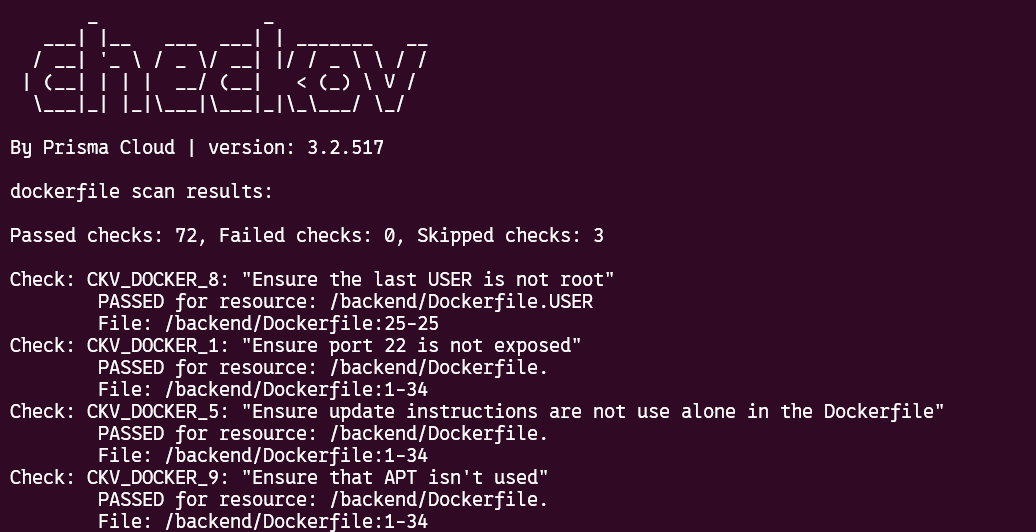
\includegraphics[width=0.8\textwidth]{Arquivos/figuras/Figura_Output_PoC_Checkov.png}
    \fonte{Elaborado pelo autor}
\end{figure}

\begin{figure}[!ht]
    \caption{Saída de \texttt{terraform plan} evidenciando a criação determinística de dez recursos (rede, banco, réplicas de aplicação e \textit{frontend}), sem alterações ou destruições -- previsibilidade requerida para o gate de aprovação.}
    \label{fig:terraform-plan-out}
    \centering
    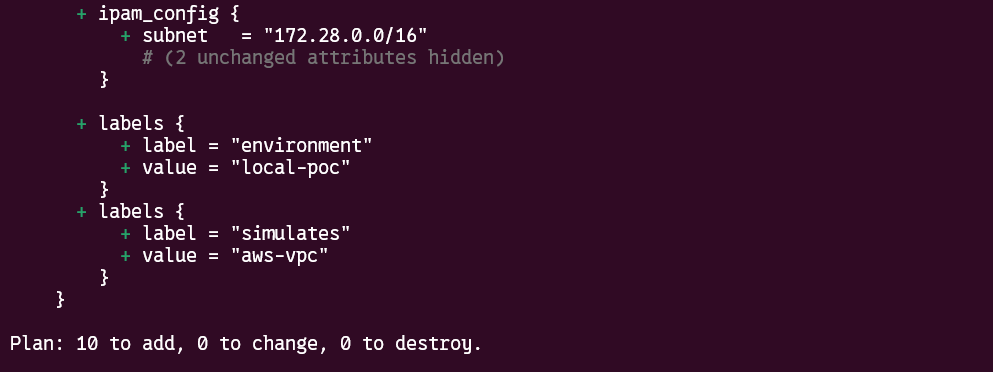
\includegraphics[width=0.8\textwidth]{Arquivos/figuras/Figura_Output_PoC_Terraform_Plan.png}
    \fonte{Elaborado pelo autor}
\end{figure}

\begin{figure}[!ht]
    \caption{Listagem \texttt{docker ps} após o provisionamento: \textit{ELB-NGINX} publicado em 3000, réplicas \textit{EKS-FASTAPI-XX} e \textit{RDS-POSTGRES}, todos em processo de inicialização (\textit{health: starting}).}
    \label{fig:docker-ps-out}
    \centering
    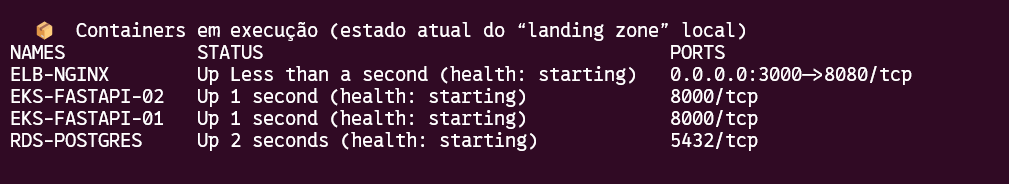
\includegraphics[width=0.8\textwidth]{Arquivos/figuras/Figura_Output_PoC_Container.png}
    \fonte{Elaborado pelo autor}
\end{figure}

\section{Ciclo de Feedback e Interrupção (\textit{Fail-Fast})}

Nas duas PoC, o princípio \textit{Fail-Fast} é aplicado de forma consistente: se qualquer \textit{gate} (segredos, análise estática, Policy-as-Code, imagem) falhar, o \textit{pipeline} é interrompido imediatamente e o desenvolvedor recebe \textit{feedback} detalhado no console do terminal e na interface do Git, com o arquivo, a linha exata do erro e o link para a documentação de remediação~\citeonline{OWASPCheatSheet}. O impacto quantitativo dessa arquitetura, medido nos testes controlados descritos na Seção~\ref{sec:testes-controlados}, é analisado no Capítulo~5.
